\providecommand{\qcOne}{\mathbf{1}}   %
\providecommand{\qcTwo}{\mathbf{2}}   %
\providecommand{\qcInt}{\mathbb{I}}   %
\providecommand{\Cat}{\mathcal{C}at}
\providecommand{\QCat}{\mathcal{Q}\mathcal{C}at}

\section{\trSmotheringFunctor}\label{sec:smothering-functors}

设 $Q$ 是一个\trQuasiCategory{}。由引理 1.1.12 回忆起，它的\trHomotopyCategory{}%
$\mathrm{h}Q$ 具有：
\begin{itemize}
\item 对象：$Q$ 的诸\trElement{}；
\item 箭头：$Q$ 的 1-\trSimplex{}的诸\trHomotopy{}类——其中平行的 1-\trSimplex{}是%
\trHomotopic{}，当且仅当它们界定一个 2-\trSimplex{}，而其余的那条外侧边退化；以及
\item 一个合成关系——当且仅当代表这三个箭头的任意一组选定的 1-\trSimplex{}都%
界定一个 2-\trSimplex{}。
\end{itemize}
对 1-\trCategory{} $J$，经典\trHomotopy{}论中众所周知：图表的\trHomotopyCategory{}%
$\mathrm{h}(Q^J)$ 并不\trEquivalence{}于\trHomotopyCategory{}中的图表之\trCategory{}%
$(\mathrm{h}Q)^J$——除非在非常特殊的情形，比如 $J$ 是一个集合时（见引理 2.3.3）。
$\mathrm{h}(Q^J)$ 的对象是 $Q$ 中形状为 $J$ 的\emph{\trHomotopy{}相干\trDiagram}，而%
$(\mathrm{h}Q)^J$ 的对象只是\emph{\trHomotopy{}交换\trDiagram}。%
然而，存在一个典范的比较函子
\[
\mathrm{h}(Q^J)\longrightarrow(\mathrm{h}Q)^J
\]
它由把 $\mathrm{h}\colon\QCat\to\Cat$ 作用于求值函子 $Q^J\times J\to Q$ 再转置而得；
\trHomotopy{}相干\trDiagram{}特别地也是\trHomotopy{}交换\trDiagram{}。

我们在本节中的第一个目标是更好地理解\trHomotopyCategory{} $\mathrm{h}Q$ 中的箭头%
与 $Q$ 的箭头——即\trQuasiCategory{}中的 1-\trSimplex{}——之间的关系。为研究这一点，
我们考察\trQuasiCategory{} $Q^{\qcTwo}$：$Q$ 的箭头作为\trElement{}居于其中，其中%
$\qcTwo=\Delta[1]$ 是行走箭头（walking arrow）的\trNerve{}。%
我们的记号有意模仿\textbf{箭头范畴}（category of arrows）的惯用记号：若 $C$ 是%
一个 1-\trCategory{}，则 $C^{\qcTwo}$ 是这样一个\trCategory{}，其对象是 $C$ 中的%
箭头，其态射是交换方块，且视作从竖放于左侧的箭头到竖放于右侧的箭头的态射。%
这一记号上的混同引出我们的第一个问题：$Q^{\qcTwo}$ 的\trHomotopyCategory{}与%
\trHomotopyCategory{} $\mathrm{h}Q$ 中的箭头范畴之间有何关系？

\begin{lemma}\label{lem:canonical-q2}
典范函子 $\mathrm{h}(Q^{\qcTwo})\to(\mathrm{h}Q)^{\qcTwo}$：
\begin{enumerate}[label=(\roman*)]
\item 对象上满射；
\item 满；以及
\item 保守——即反射态射的可逆性，%
\end{enumerate}
但未必对象上单，也未必忠实。
\end{lemma}

\begin{proof}
对象上的满射断言：\trHomotopyCategory{} $\mathrm{h}Q$ 中的每个箭头都由 $Q$ 中的%
一个 1-\trSimplex{}所代表。这正是练习 1.1.iii(iii) 的结论，该练习概述了引理%
1.1.12 的证明。
为证满性，考察 $Q$ 中的一对箭头 $f$ 与 $g$，它们构成 $\mathrm{h}Q$ 中某个交换%
方块的源与目标。据 (i)，我们可以任取代表 $\mathrm{h}Q$ 中各态射及其公共合成的%
1-\trSimplex{}：
\begin{center}
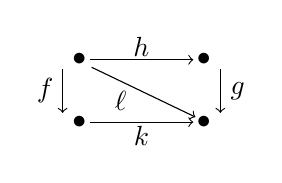
\begin{tikzpicture}[x=1.5em,y=1.5em]
  \node (tl) at (0,1.5) {$\bullet$};
  \node (tr) at (3,1.5) {$\bullet$};
  \node (bl) at (0,0) {$\bullet$};
  \node (br) at (3,0) {$\bullet$};
  \draw[->] (0.25,1.5) -- (2.75,1.5);
  \node at (1.5,1.82) {$h$};
  \draw[->] (-0.4,1.28) -- (-0.4,0.22);
  \node at (-0.82,0.75) {$f$};
  \draw[->] (3.4,1.28) -- (3.4,0.22);
  \node at (3.82,0.75) {$g$};
  \draw[->] (0.25,0) -- (2.75,0);
  \node at (1.5,-0.34) {$k$};
  \draw[->] (0.3,1.32) -- (2.8,0.12);
  \node at (1.0,0.52) {$\ell$};
\end{tikzpicture}
\end{center}
由引理 1.1.12，$\mathrm{h}Q$ 中的每个合成关系都由 $Q$ 中的一个 2-\trSimplex{}见证；%
选取一对这样的 2-\trSimplex{}便定义了一个图表 $\qcTwo\times\qcTwo\to Q$，它代表%
$\mathrm{h}(Q^{\qcTwo})$ 中一个从 $f$ 到 $g$ 的态射，满性得证。
函子 $\mathrm{h}(Q^{\qcTwo})\to(\mathrm{h}Q)^{\qcTwo}$ 的对象满射性与满性是与\trDiagram{}%
形状 $\qcTwo$ 相关的特殊性质，而保守性据推论 1.1.22 对一般的\trDiagram{}形状成立。
展示对象单性与忠实性普遍失效的反例之构造留作\cref{ex:smothering-counterexample}，%
并附有提示。
\end{proof}

典范函子 $\mathrm{h}(Q^{\qcTwo})\to(\mathrm{h}Q)^{\qcTwo}$ 的这些性质将反复出现，
故我们以一个发人联想的名字为它们命名：

\begin{definition}[\trSmotheringFunctor]\label{def:smothering-functor}
1-\trCategory{}之间的\trFunctor{} $f\colon A\to B$ 是\textbf{\trSmothering}（smothering），%
若它在对象上满射、满且保守。也就是说，一个\trFunctor{}是\trSmothering{}，当且仅当它对%
下列\trFunctor{}之集具有右提升性质：
\[
\left\{\;
\mbox{\begin{tikzpicture}[x=1.2em,y=1.2em]
  \node (a) at (0,0.9) {$\varnothing$};
  \node (b) at (0,-0.9) {$\qcOne$};
  \draw[->] (0,0.5) -- (0,-0.5);
  \draw (0,0.5) arc[start angle=180,end angle=0,radius=0.15];
\end{tikzpicture}}
\;,\;
\mbox{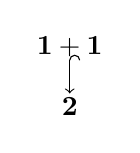
\begin{tikzpicture}[x=1.2em,y=1.2em]
  \node (a) at (0,0.9) {$\qcOne+\qcOne$};
  \node (b) at (0,-0.9) {$\qcTwo$};
  \draw[->] (0,0.5) -- (0,-0.5);
  \draw (0,0.5) arc[start angle=180,end angle=0,radius=0.15];
\end{tikzpicture}}
\;,\;
\mbox{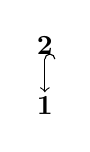
\begin{tikzpicture}[x=1.2em,y=1.2em]
  \node (a) at (0,0.9) {$\qcTwo$};
  \node (b) at (0,-0.9) {$\qcOne$};
  \draw[->] (0,0.5) -- (0,-0.5);
  \draw (0,0.5) arc[start angle=180,end angle=0,radius=0.15];
\end{tikzpicture}}
\;\right\}
\]
\end{definition}

\cref{ex:smothering-properties}建立了覆盖函子的诸多初等性质；这里我们强调其中%
一条值得特别留意的：

\begin{lemma}[\trSmotheringFunctor{}的\trFiber]\label{lem:smothering-fibers}
覆盖函子的每条\trFiber{}都是非空连通\trGroupoid{}。
\end{lemma}

\begin{proof}
设 $f\colon A\to B$ 是\trSmothering{}，考察 $B$ 中对象 $b$ 上的\trFiber{}：
\begin{center}
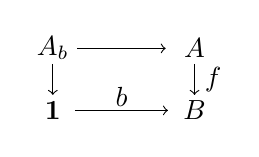
\begin{tikzpicture}[x=1.6em,y=1.6em]
  \node (tl) at (0,1.4) {$A_b$};
  \node (tr) at (3.2,1.4) {$A$};
  \node (bl) at (0,0) {$\qcOne$};
  \node (br) at (3.2,0) {$B$};
  \draw[->] (0.55,1.4) -- (2.55,1.4);
  \draw[->] (0,1.05) -- (0,0.35);
  \node at (0.45,0.78) {$\scriptstyle\lrcorner$};
  \draw[->] (3.2,1.05) -- (3.2,0.35);
  \node at (3.62,0.7) {$f$};
  \draw[->] (0.5,0) -- (2.6,0);
  \node at (1.55,0.3) {$b$};
\end{tikzpicture}
\end{center}
由对象上的满射性，\trFiber{}非空。\trFiber{}中的态射定义为 $b$ 的\trFiber{}中对象之间、且映到%
$b$ 上恒同的箭头。由满性，\trFiber{}中的任意两个对象都由一个态射相连，甚至由指向%
两个方向的态射相连。由保守性，\trFiber{}中的所有态射都必然是\trInvertible{}。
\end{proof}

用于证明\cref{lem:canonical-q2}的论证可推广为：

\begin{lemma}\label{lem:smothering-free}
若 $J$ 是一个在\trReflexiveDirectedGraph{}上\trFree 1-\trCategory{}，而 $Q$ 是一个%
\trQuasiCategory{}，则典范函子 $\mathrm{h}(Q^J)\to(\mathrm{h}Q)^J$ 是\trSmothering{}。
\end{lemma}
\begin{proof}
见\cref{ex:smothering-free}。
\end{proof}

\trCotensor{}是定义 1.2.1 所公理化的诸\trCosmologicalLimitNotions{}之一。
那里列出的其他\trLimit{}构造也给出覆盖函子。

\begin{lemma}\label{lem:smothering-pullback}
对由\trQuasiCategory{}构成的任何\trPullback{}图表，其中 $p$ 是\trIsofibration{}：
\begin{center}
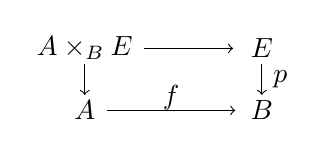
\begin{tikzpicture}[x=1.6em,y=1.6em]
  \node (tl) at (0,1.4) {$A\times_BE$};
  \node (tr) at (4.0,1.4) {$E$};
  \node (bl) at (0,0) {$A$};
  \node (br) at (4.0,0) {$B$};
  \draw[->] (1.35,1.4) -- (3.35,1.4);
  \draw[->] (0,1.05) -- (0,0.35);
  \node at (0.45,0.78) {$\scriptstyle\lrcorner$};
  \draw[->] (4.0,1.05) -- (4.0,0.35);
  \node at (4.42,0.7) {$p$};
  \draw[->] (0.5,0) -- (3.4,0);
  \node at (1.95,0.3) {$f$};
\end{tikzpicture}
\end{center}
典范函子 $\mathrm{h}(A\times_BE)\to\mathrm{h}A\times_{\mathrm{h}B}\mathrm{h}E$ 是\trSmothering{}。
\end{lemma}
\begin{proof}
由于 $\mathrm{h}\colon\QCat\to\Cat$ 不保持\trPullback{}，题中的典范比较函子不是%
\trIsomorphism{}。但它对象上双射，因为复合函子
\[
\QCat\xrightarrow{\;\mathrm{h}\;}\Cat\xrightarrow{\;\mathrm{obj}\;}\mathcal{S}et
\]
落到每个\trQuasiCategory{}的底层顶点集上，且该函子\emph{确实}保持\trPullback{}。

为证满性，注意 $\mathrm{h}A\times_{\mathrm{h}B}\mathrm{h}E$ 中的态射由一对%
1-\trSimplex{}代表——$A$ 中的 $\alpha\colon a\to a'$ 与 $E$ 中的%
$\epsilon\colon e\to e'$，它们的像在 $B$ 中\trHomotopic——这一条件特别地蕴含%
$f(a)=p(e)$ 与 $f(a')=p(e')$。

由引理 1.1.9，我们可以随心所欲地配置这一\trHomotopy{}，于是选取 2-\trSimplex{}%
见证者 $\beta$，以定义如下的\trLifting{}问题
\begin{center}
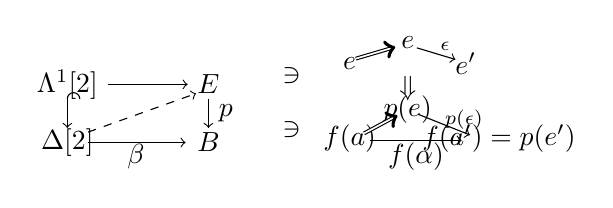
\begin{tikzpicture}[x=1.5em,y=1.5em]
  \node (tl) at (0,1.4) {$\Lambda^1[2]$};
  \node (tr) at (3.4,1.4) {$E$};
  \node (bl) at (0,0) {$\Delta[2]$};
  \node (br) at (3.4,0) {$B$};
  \draw[->] (tl) -- (tr);
  \draw[->] (0,1.05) -- (0,0.35);
  \draw (0,1.05) arc[start angle=180,end angle=0,radius=0.15];
  \draw[->] (3.4,1.05) -- (3.4,0.35);
  \node at (3.82,0.7) {$p$};
  \draw[->] (0.5,0) -- (2.85,0);
  \node at (1.65,-0.35) {$\beta$};
  \draw[->,dashed] (0.5,0.25) -- (3.1,1.18);
  \node at (5.4,1.6) {$\ni$};
  \node (e0) at (6.8,1.9) {$e$};
  \node (e1) at (8.2,2.4) {$e$};
  \node (e2) at (9.6,1.9) {$e'$};
  \draw[double,->] (6.95,2.02) -- (7.9,2.3);
  \draw[->] (8.42,2.28) -- (9.35,2.0);
  \node at (9.1,2.32) {$\scriptstyle\epsilon$};
  \node at (8.2,1.3) {$\Downarrow$};
  \node at (5.4,0.3) {$\ni$};
  \node (fa) at (6.8,0.1) {$f(a)$};
  \node (pe) at (8.2,0.8) {$p(e)$};
  \node (fp) at (10.4,0.1) {$f(a')=p(e')$};
  \draw[double,->] (7.15,0.22) -- (7.95,0.65);
  \draw[->] (8.45,0.68) -- (9.7,0.18);
  \node at (9.55,0.55) {$\scriptstyle p(\epsilon)$};
  \draw[->] (7.3,0.05) -- (9.5,0.05);
  \node at (8.4,-0.35) {$f(\alpha)$};
\end{tikzpicture}
\end{center}
由于 $p$ 是\trIsofibration{}，解存在，它定义了 $E$ 中与 $\epsilon$ 属同一%
\trHomotopy{}类的一条箭头 $\tilde{\epsilon}\colon e\to e'$，使得%
$p(\tilde{\epsilon})=f(\alpha)$。数对 $(\alpha,\tilde{\epsilon})$ 现在便定义了%
$\mathrm{h}(E\times_BA)$ 中所提升的那条箭头。

最后，考虑一条箭头 $\qcTwo\to A\times_BE$，它在 $\mathrm{h}A\times_{\mathrm{h}B}\mathrm{h}E$ 中的像是\trIsomorphism——这只在到 $E$ 与到 $A$ 的投影都定义%
\trIsomorphism{}时发生。由推论 1.1.16，我们可以选取一个%
\trHomotopyCoherentIsomorphism{} $\qcInt\to A$，扩张给定的\trIsomorphism{}%
$\qcTwo\to A$。这份数据向我们呈现如下\trLifting{}问题
\begin{center}
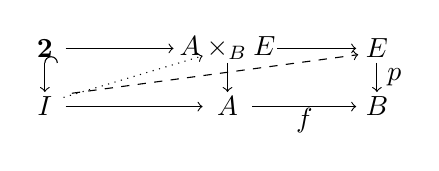
\begin{tikzpicture}[x=1.5em,y=1.5em]
  \node (tl) at (0,1.4) {$\qcTwo$};
  \node (tm) at (4.4,1.4) {$A\times_BE$};
  \node (tr) at (8.0,1.4) {$E$};
  \node (bl) at (0,0) {$\qcInt$};
  \node (bm) at (4.4,0) {$A$};
  \node (br) at (8.0,0) {$B$};
  \draw[->] (0.5,1.4) -- (3.1,1.4);
  \draw[->] (5.6,1.4) -- (7.5,1.4);
  \draw[->] (0,1.05) -- (0,0.35);
  \draw (0,1.05) arc[start angle=180,end angle=0,radius=0.15];
  \draw[->] (4.4,1.05) -- (4.4,0.35);
  \node at (4.85,0.82) {$\scriptstyle\lrcorner$};
  \draw[->] (8.0,1.05) -- (8.0,0.35);
  \node at (8.42,0.7) {$p$};
  \draw[->] (0.5,0) -- (3.8,0);
  \draw[->] (5.0,0) -- (7.5,0);
  \node at (6.25,-0.35) {$f$};
  \draw[->,dotted] (0.45,0.22) -- (3.8,1.22);
  \draw[->,dashed] (0.65,0.32) -- (7.55,1.25);
\end{tikzpicture}
\end{center}
而练习 1.1.vi 告诉我们它可以求解。
这便证明了 $\mathrm{h}(A\times_BE)\to\mathrm{h}A\times_{\mathrm{h}B}\mathrm{h}E$ 是%
\trConservative{}，从而也是\trSmothering{}。
\end{proof}

类似的论证可证明：

\begin{lemma}\label{lem:smothering-tower}
对\trQuasiCategory{}之间的任何\trIsofibration{}之塔
\[
\cdots\twoheadrightarrow E_n\twoheadrightarrow E_{n-1}\twoheadrightarrow\cdots
\twoheadrightarrow E_2\twoheadrightarrow E_1\twoheadrightarrow E_0
\]
典范函子 $\mathrm{h}(\lim_n E_n)\to\lim_n\mathrm{h}E_n$ 是\trSmothering{}。
\end{lemma}
\begin{proof}
见\cref{ex:smothering-tower}。
\end{proof}

\begin{lemma}\label{lem:smothering-hom}
对\trQuasiCategory{}之间的任何余跨度 $C\xrightarrow{\;g\;}A\xleftarrow{\;f\;}B$，
考察由如下\trPullback{}定义的\trQuasiCategory
\begin{center}
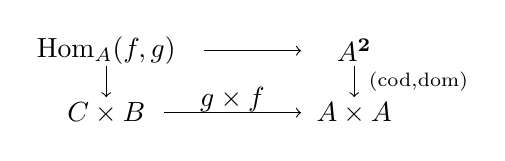
\begin{tikzpicture}[x=1.6em,y=1.6em]
  \node (tl) at (0,1.4) {$\mathrm{Hom}_A(f,g)$};
  \node (tr) at (5.6,1.4) {$A^{\qcTwo}$};
  \node (bl) at (0,0) {$C\times B$};
  \node (br) at (5.6,0) {$A\times A$};
  \draw[->] (2.2,1.4) -- (4.4,1.4);
  \draw[->] (0,1.05) -- (0,0.35);
  \node at (0.45,0.78) {$\scriptstyle\lrcorner$};
  \draw[->] (5.6,1.05) -- (5.6,0.35);
  \node at (7.05,0.7) {$\scriptstyle(\mathrm{cod},\mathrm{dom})$};
  \draw[->] (1.3,0) -- (4.4,0);
  \node at (2.85,0.3) {$g\times f$};
\end{tikzpicture}
\end{center}
典范函子 $\mathrm{h}\mathrm{Hom}_A(f,g)\to\mathrm{Hom}_{\mathrm{h}A}(\mathrm{h}f,\mathrm{h}g)$%
是\trSmothering{}。
\end{lemma}

\begin{proof}
该函子的余域是由 $\Cat$ 中一个类似的\trPullback{}所定义的\trCategory
\begin{center}
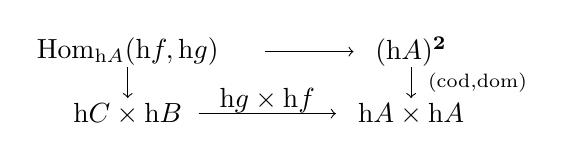
\begin{tikzpicture}[x=1.6em,y=1.6em]
  \node (tl) at (0,1.4) {$\mathrm{Hom}_{\mathrm{h}A}(\mathrm{h}f,\mathrm{h}g)$};
  \node (tr) at (6.4,1.4) {$(\mathrm{h}A)^{\qcTwo}$};
  \node (bl) at (0,0) {$\mathrm{h}C\times\mathrm{h}B$};
  \node (br) at (6.4,0) {$\mathrm{h}A\times\mathrm{h}A$};
  \draw[->] (3.1,1.4) -- (5.1,1.4);
  \draw[->] (0,1.05) -- (0,0.35);
  \node at (0.45,0.78) {$\scriptstyle\lrcorner$};
  \draw[->] (6.4,1.05) -- (6.4,0.35);
  \node at (7.9,0.7) {$\scriptstyle(\mathrm{cod},\mathrm{dom})$};
  \draw[->] (1.6,0) -- (4.7,0);
  \node at (3.15,0.3) {$\mathrm{h}g\times\mathrm{h}f$};
\end{tikzpicture}
\end{center}
而该典范函子分解为
\[
\mathrm{h}\mathrm{Hom}_{A}(f,g)\longrightarrow
\mathrm{h}(A^{\qcTwo})\times_{\mathrm{h}A\times\mathrm{h}A}(\mathrm{h}C\times\mathrm{h}B)
\longrightarrow
(\mathrm{h}A)^{\qcTwo}\times_{\mathrm{h}A\times\mathrm{h}A}(\mathrm{h}C\times\mathrm{h}B)
\]
由\cref{lem:smothering-pullback}，这些函子中的第一个是\trSmothering{}。由%
\cref{lem:canonical-q2}，第二个是某个覆盖函子的\trPullback{}。于是据%
\cref{ex:smothering-properties}(i)可得：复合函子是\trSmothering{}。
\end{proof}

在接下来的几节中，我们将发现：刚刚构造的这些覆盖函子表达了任何%
\trInfinityCosmos{}的\trHomotopyTwoCategory{}中箭头、\trPullback{}与逗号构造的%
弱\trUniversalProperty{}。

\subsection*{练习}

\begin{exercise}\label{ex:smothering-counterexample}
找一个显式的例子：一个\trQuasiCategory{} $Q$，使得典范覆盖函子%
$\mathrm{h}(Q^{\qcTwo})\to(\mathrm{h}Q)^{\qcTwo}$ 在对象上不单、也不忠实——%
例如取 $Q$ 为某个适当拓扑空间的总奇异复形。
\end{exercise}

\begin{exercise}\label{ex:smothering-properties}
证明：
\begin{enumerate}[label=(\roman*)]
\item 覆盖函子在复合、\trRetract{}、\trProduct{}、\trPullback{}与塔的\trLimit{}下封闭。
\item \trCategory{}之间的\trSurjectiveEquivalence{}是覆盖函子。
\item 覆盖函子是\trIsofibration{}，也就是说，是对 $\qcOne\hookrightarrow\qcInt$ 具有%
右提升性质的映射。
\item 证明：若 $f$ 与 $gf$ 是覆盖函子，则 $g$ 是覆盖函子。\footnote{事实上，%
只需假设 $f$ 在对象与箭头上满射便已足够。}
\end{enumerate}
\end{exercise}

\begin{exercise}\label{ex:smothering-free}
证明\cref{lem:smothering-free}。
\end{exercise}

\begin{exercise}\label{ex:smothering-tower}
证明\cref{lem:smothering-tower}。
\end{exercise}
